% !TEX encoding = UTF-8 Unicode

\chapter*{ВВЕДЕНИЕ}
\addcontentsline{toc}{chapter}{ВВЕДЕНИЕ}
Данный отчет по научной работе посвящен теории восстановления и моделированию процессов восстановления на компьютере.

{\bfseries Теория восстановления} - это раздел теории вероятности, описывающий широкий круг явлений, связанных с отказом и восстановлением элементов какой-либо системы. Основными понятиями теории восстановления являются процесс восстановления и уравнение восстановления.

Под  \textit { процессом восстановления} мы понимаем последовательность неотрицательных, взаимно независимых случайных величин \{$X_n$, n = 1, 2, ...\}, которые для $n\ge2$ одинаково распределены. Процесс восстановления называется \textit{ запаздывающим }, если $F_1(t) \neq F(t)$, и соответственно \textit{обычным}, если $F_1(t)=F(t)$.

\textit{Функцией восстановления} называется функция вида\\ $H_1(t)=E(N(t))$. В части анализа данная функция будет рассмотрена подробнее.

Теория восстановления, как было сказано ранее, относиться к теории вероятности и позволяет произвести расчет необходимых запчастей для стабильной работы системы, следственно является актуальной и применимой на сегодняшний день.
\newpage
\chapter*{ПОСТАНОВКА ЗАДАЧИ}
\addcontentsline{toc}{chapter}{ПОСТАНОВКА ЗАДАЧИ}
В рамках научной работы передо мной были поставлены следующие задачи:\\
\begin{enumerate}
\item Изучить основы теории восстановления
\item Изучить альтернирующие  процессы восстановления
\item Изучить моделирование случайных процессов
\item Изучить необходимые средства разработки для написания программы
\item Смоделировать процесс восстановления для случайных процессов распределенных по следующим законам:
\begin{itemize}
\item Гамма распределение
\item Нормальное распределение
\item Распределение Вейбула-Гнеденко
\end{itemize}
\item Решить методом конечных сумм интегральное уравнение восстановления для вышеперечисленных процессов
\item Вычислить для альтернирующего процесса заданного по двум выбранным законам следующие коэффициенты:
\begin{itemize}
\item нестационарный/стационарный коэффициент готовности
\item нестационарный/стационарный оперативный коэффициент готовности
\end{itemize}
\end{enumerate}
\newpage
\chapter*{ОСНОВНАЯ ЧАСТЬ}
\addcontentsline{toc}{chapter}{ОСНОВНАЯ ЧАСТЬ}
Как было сказано в введении, в данной работе будет вестись об основах моделирования процессов восстановления. 
В данной части будут рассмотрены математический аппарат и базовая теория необходимая для выполнения задачи. Так же будут рассмотрены средства разработки которые были использованы для написания программы отвечающей условиям поставленной задачи. Начнем с математической части работы.
\begin{center}
\section{Анализ}
\subsection{Основы теории восcтановления}
\end{center}
Сперва введем список основных обозначений:

\begin{description}
\item[$X_k$] наработка после $(k-1)$-го восстановления
\item[$T_k$] момент k-ого восстановления
\item[N(t)] считающий процесс восстановления
\item[$F_1(t), F(t)$] функции распределения соответственно для $X_1$ и $X_k, k \geqslant 2$
\item[$f_1(t), f(t)$] плотности распределения, соответствующие функциям $F_1$ и $F$
\item[$H_1(t), H(t)$] $E(N(t))$, функция восстановления запаздывающего(обычного) процесса восстановления
\item[$h_1(t), h(t)$] плотности восстановления
\end{description}

Данные обозначения для теории восстановления вводятся Байхельтом Франкеном для теории восстановления. Теперь перейдем непосредственно  к рассмотрению основ теории восстановления.

Как было сказано еще в введении, процессы восстановления делятся на две группы: запаздывающие и обычные. Различие в них только от начального состояния при котором начинается моделирование. Особый интерес в моделировании процесса восстановления представляет собой \textit{считающий процесс восстановления}:
\begin{equation}
N(t) = max\{k: T_k \leqslant t\}, N(t) = 0 \text{ для } t < T_1.
\end{equation}

Таким образом, для каждого момента $t$ величина $N(t)$ означает случайное число восстановлений, произошедших за время $[0, t]$. Из выражения (1) немедленно следует, что неравенство $T_k \leqslant t$ выполняется тогда и только тогда, когда $N(t) \geqslant k$.  Поэтому
\begin{equation}
F_k(t) = P(T_k \leqslant t) = P(N(t) \geqslant k),
\end{equation}
причем функция распределения $F_k(t)$ величины $T_k$ из-за независимости случайных величин $X_k$ для $k \geqslant 1$ задается формулой
\begin{equation}
F_k(t) = F_1 * F^{*(k-1)}(t), t \geqslant 0,
\end{equation}
где $F^{*(0)}(t) = 1$. Если существуют плотности $f_1(t) = F'_1(t)$ и $f(t) = F'(t)$, то соответствующие (3) плотности распределения имеют вид
\begin{equation}
f_k = f_1 * f^{*(k-1)}(t), t \geqslant 0.
\end{equation}

Следующим важным понятием в теории восстановления является \textit{функция восстановления ($H(t) = E(N(t))$)}, определение которой было дано в введении. По определению математического ожидания:

$H_1(t) = \sum\limits_{k=1}^\infty F_1* F^{*(k-1)}(t) = \sum\limits_{k=1}^\infty P(N(t) \geqslant k).$

Из соотношений (2) и  (3) следует:
\begin{equation}
H_1(t) = \sum\limits_{k=1}^\infty F_1 * F^{*(k-1)}(t).
\end{equation}

Подставляя в  (5) выражение:

$F_1 * F^{*k}(t) = \int\limits_0^t F_1 * F^{*(k-1)}(t-x) dF(x)$

получим:

$H_1(t) = F_1(t) + \sum\limits_{k=1}^\infty \int\limits_0^t F_1 * F^{*(k-1)}(t-x) dF(x).$

Меняя порядок суммирования и интегрирования, получим для нее интегральное уравнение
\begin{equation}
H_1(t) = F_1(t) + \int\limits_0^t H_1(t-x) dF(x).
\end{equation}

Замена свертки $F_1 * F^{*(k)}(t)$ на $\int\limits_0^t F^{*(k)}(t-x) dF_1(x)$ дает
\begin{equation}
H_1(t) = F_1(t) + \int\limits_0^t H(t-x) dF_1(x),
\end{equation}
где $H(t)$ - функция восстановления простого процесса восстановления. Согласно (6) функция H(t) удовлетворяет интегральному уравнению
\begin{equation}
H(t) = F(t) + \int\limits_0^t H(t-x) dF(x).
\end{equation}

Соотношения (6)-(8) называются \textit{уравнениями восстановления}. Они имеют единственное решение.

Если существуют плотности распределений, то из (6)-(8) получаются соответствующие уравнения
\begin{equation}
h_1(t) = \sum\limits_{k=1}^\infty f_1 * f^{*(k-1)},
\end{equation}

\begin{equation}
h_1(t) = f_1(t) + \int\limits_0^t h_1(t-x) f(x) dx,
\end{equation}

\begin{equation}
h_1(t) = f_1(t) + \int\limits_0^t h(t-x) f_1(x) dx,
\end{equation}

\begin{equation}
h(t) = f(t) + \int\limits_0^t h(t-x) f(x) dx.
\end{equation}

Уравнения (6)-(8) и (10)-(12) решаются численными методами. В данной работе для решения данных уравнений применим метод конечных сумм.

\begin{center}
\item\subsection{Альтернирующие процессы восстановления}
\end{center}

В предыдущей части мы рассматривали процессы восстановления для которых само время замены/восстановления пренебрежительно мало. В реальном мире такие процессы встречаются крайне редко. Поэтому введем вторую случайную величину - $Y_i$ . $Y_i$ - время затраченное на восстановление после i-го отказа Моменты времени $T_1 = X_1$, $T_2 = X_1 + Y_1 + X_2$,... , в которые система отказывает, называют моментами отказов или моментами \textit{0-восстановлений}, а моменты времени времени $S_1 = X_1 + Y_1$, $S_2 = X_1 + Y_1 + X_2 + Y_2$,... , в которые заканчивается восстановления - моментами восстановления (или \textit{1-восстановлениями}).

Введем понятие \textit{альтернируещего процесса}. Если $\{X_n, n \geqslant 1\}$ и $\{Y_n, n \geqslant 1\}$ - две последовательности независимых одинаково распределенных не отрицательных случайных величин,  то последовательность $\{ (X_n, Y_n), n \geqslant 1 \}$, так же как последовательность и последовательность $\{ (Y_k, S_k), k \geqslant 1 \}$, называется \textit{альтерирующим процессом восстановления}.  Так же, приведенный выше, процесс восстановления можно эквивалентным образом описать процессом $\{ Z(t), t \geqslant 0 \}$ с помощью соотношения
\begin{equation}
Z(t) = 
\begin{cases}
0, \text{если} t\in[T_x, S_k),\\
1, \text{в противном случае},
\end{cases}
\end{equation}
поскольку  реализации процесса $\{ (X_n, Y_n) \}$ или $\{ T_k, S_k \}$ взаимно однозначно определяются по реализациям процесса $\{Z(t)\}$. В дальнейшем будем рассматривать исключительно альтернирующие процессы восстановления в смысле приведенного определения. В этом случае $P(Z(+0) = 1) = 1$.

Через $N_0(t)$ обозначим случай число 0-восстановлений, а через $N_1(t)$ случайное число 1-восстановлений на интервале $(0,t]$. Очевидно, $N_0(t)$ и $N_1(t)$ являются считающими альтернирующими процессами, которые определяются функциями распределения $F(t)$ и $(G*F)(t)$, так что можно применять результаты разд. 1.1 - 1.6. Согласно формулам (1.2) и  (1.3) справедливы соотношения

\begin{equation}
P(N_0(t) \geqslant k) = P(T_k \leqslant t) = F * (G * F)^{*(k-1)}(t);
\end{equation}

\begin{equation}
P(N_1(t) \geqslant k) = P(S_k \leqslant t) = (F * G)^{*(k)}(t).
\end{equation}
Отсюда средние значения 0- и 1-восстановлений на интервале задаются функциями восстановления
\begin{equation}
H_0(t) = E(N_0(t)) = \sum_{k=1}^\infty F * (G * F)^{*(k-1)}(t)
\end{equation}
и
\begin{equation}
H_1(t) = E(N_1(t)) = \sum_{k=1}^\infty (F * G)^{*(k)}(t).
\end{equation}

Особый интерес представляют вероятности  $P(Z(t) = i, V_t^{(i)} > x). i = 1, 2$, где $V_t^{(1)}$ означает остаточную наработку, а $V_t^{(2)}$ - остаточное время восстановления. Очевидно $P(Z(t)) = 1, V_t^{(1)} > x$ означает вероятность того, что исправная к моменту $t$ система не откажет на следующем интервале времени $(t, t+x]$. С учетом (13) по формуле полной вероятности получаем\\
$P(Z(t) = 1, V_t^{(1)} > x) = P(t + x > X_1) + \sum_{k=1}^\infty P(S_k < t, t + x < S_k + X_{k+1}) =  \overline{F}(t + x) + \sum_{k = 1}^\infty \int_0^t P(t + x < u + X_{k+1}) d(F * G)^{*(k)}(u)$.

Из (17) следует
\begin{equation}
P(Z(t) = 1, V_t^{(1)} > x) = \overline{F}(t + x) + \int_0^t\overline{F}(t + x - u) dH_1(u).
\end{equation}
Это так называемый \textit{нестационарный коэффициент оперативной гтовности} для альтернирующего  процесса восстановления. \textit{Нестационарный коэффициент готовности} определяется соотношением
\begin{equation}
K(t) = P(Z(t) = 1) = E(Z(t)).
\end{equation}
Он равен вероятности того, что система работает в момент $t$.  Если положить в соотношении (17) $x = 0$, то для этого частного случая
\begin{equation}
K(t) = \overline{F}(t) + \int_0^t \overline{F}(t - u) dH_1(u).
\end{equation}

Нестационарный средний коэффициент готовности определяется соотношением\\
$\check{K}(t) = \frac{1}{t} \int_0^t K(u) du$.

Согласно (20) $K(t)$ можно представить в следующем виде:
\begin{equation}
\check{K}(t) = \frac{1}{t}\int_0^t \overline{F}(u) du + \frac{1}{t}\int_0^t(H_1(u) - (F * H_1)(u)) du.
\end{equation}

 \begin{equation}
 K_x(t) = \int_0^t (1 - F(t+x-u)) dH_1
 \end{equation}
 
  \begin{equation}
 K_x(t) = 1 - F(t+x) + \int_0^t K_x(t - u) f*g(u) du
 \end{equation}

{\bfseries Теорема.} Пусть функция распределения $(F * G)(t)$ не является арифметической и пусть $\mu + \nu < \infty$, где \\
$\mu = \int_0^\infty \overline{F}(u) du, \nu = \int_0^\infty \overline{G}(u) du$.\\
Тогда справедливы соотношения
\begin{equation}
K_x = \lim_{t \to \infty}P(Z(t) = 1, V_t^{(1)} > x) = \frac{1}{\mu + \nu}\int_0^\infty \overline{F}(u) du;
\end{equation} 
\begin{equation}
K = \lim_{t \to \infty}K(t) = \lim_{t \to \infty} \frac{1}{t}\int_0^t K(u) du = \mu/(\mu + \nu).
\end{equation}

$K_x$ и $K$ называются \textit{(стационарным) коэффициентом оперативной готовности} и \textit{(стационарным) коэффициентом готовности}.

Формулу (22) можно записать и так:
\begin{equation}
K_x = K(1 - F_R(x)).
\end{equation}

Из соотношений (22) и (24) следует элементарная оценка для коэффициента оперативной готовности:\\
$K_x \geqslant 1 - (x + \nu)/(\mu + \nu)$.

Полезные характеристики можно получить для процесса, описывающего состояние системы: $\{ Z(t), t \geqslant 0 \}$. Это прежде всего \textit{суммарное время безлткатной работы U(t)} и  \textit{суммарное время простоя D(t)} за интервал $(0, t]$:
\begin{equation}
U(t) = \int_0^t Z(u) du, D(t) = t - U(t) = \int_0^t (1 - Z(u)) du.
\end{equation}

При изучении случайных величин $U(t)$ и $D(t)$ нередко привлекают также связанные с ними величины
\begin{equation}
B_1(t) = \min\{x : U(x) \geqslant t\}, B_2(t) = B_1(t) - t,
\end{equation}
$B_1(t)$ задает случайный момент,  в  который суммарное время безоткатной работы достигает величины $t$, а $B_2(t)$ равняется времени простоя на интервале $(0, B_1(t)]$.
%Причем величина  $B_1(t)$ задает случайный момент,  в  который суммарное время безоткатной работы достигает величины $t$, а $B_2(t)$ равняется времени простоя на интервале $(0, B_1(t)]$.

\begin{center}
\item\subsubsection{Модель совместного потока}
\end{center}
Данная модель отличается от обычного альтернируещего процесса восстановления тем что 0-восстановления и 1-восстановления происходят в двух различных потоках, т.е. мы имеем не один процесс в котором чередуются 0 и 1 - восстановления, а два независимых процесса: 0-восстановлений и 1-восстановлений. Обозначим $\mu_{0,i}$ как i-ое 0-восстановление и $\mu_{1,i}$ - i-ое 1-восстановление.

Процесс 0-восстановлений ${\mu_{0,i}, i = 0,1,2, ...}$ образован случайными величинами $\Delta_1, \Delta_2, ...$, т.е. временами работы системы, при этом предполагается мгновенное восстановление:
\begin{equation}
\mu_{0,i} = \sum_{j=1}^i \Delta_j, j >0, \mu_{0,0} = 0.
\end{equation}

Аналогично ему процесс 1-восстановлений ${\mu_{1,i}, i = 0,1,2, ...}$ образован случайными величинами $\epsilon_1, \epsilon_2, ...$ - временами восстановлений работоспособности системы. Так же предполагается что отказы происходят мгновенно после восстановления системы:
\begin{equation}
\mu_{1,i} = \sum_{j=1}^i \epsilon_j, j >0, \mu_{1,0} = 0.
\end{equation}

\textit{Совместным потоком} событий (0-, 1-восстановлений) называется совокупность двух потоков - потока отказов(${\mu_{0,i}, i = 0,1,2, ...}$) и  потока восстановлений (${\mu_{1,i}, i = 0,1,2, ...}$).

\textit{Считающей функцией пар} совместного потока событий называется
\begin{equation}
\xi_{t_0,t_1} = \sum_{i=0}^\infty I\{\mu_{0,i} \leqslant t_0; \mu_{1,i} \leqslant t_1\}.
\end{equation}

\textit{Считающей функцией пар со сдвигом} (числа отказов на 1) совместного потока событий называется
\begin{equation}
\xi_{t_0,t_1} ^+= \sum_{i=0}^\infty I\{\mu_{0,i+1} \leqslant t_0; \mu_{1,i} \leqslant t_1\}.
\end{equation}

\textit{Ведущей функцией} пар совместного потока событий называется функция
\begin{equation}
\Lambda(t_0,t_1) = M\xi_{t_0,t_1} = \sum_{i=0}^\infty F_{\mu_{0,i}, \mu_{1,i}}(t_0,t_1).
\end{equation}

Ведущая функция пар со сдвигом совместного потока событий определяется аналогично считающей функции со сдвигом.

\textit{Интенсивностью потока пар} совместного потока событий, при условии существования необходимых производных, называется
 \begin{equation}
\omega(t_0, t_1) = \frac{\partial^2\Lambda(t_0, t_1)}{\partial t_0 \partial t_1} = \sum_{i=0}^\infty f_{\mu_{0,i}, \mu_{1,i}}(t_0, t_1).
\end{equation}

Свойства параметров совместного потока событий:
\begin{enumerate}
\item $ \Lambda(t_0, t_1),  \Lambda^+(t_0, t_1)$ - неубывающие функции по каждому аргументу.

\item $\lim_{t_0 \to \infty} \Lambda(t_0, t_1) = \lim_{t_0 \to \infty} \Lambda^+(t_0, t_1) = \Lambda_{\mu_0}(t_0) = \sum_{i=0}^\infty F_{\mu_{0,i}}(t_0)$ - функция восстановления автономного потока восстановлений

\item $\lim_{t_1 \to \infty} \Lambda(t_0, t_1) = 1 + \lim_{t_1 \to \infty} \Lambda^+(t_0, t_1) = \Lambda_{\mu_1}(t_1) = \sum_{i=0}^\infty F_{\mu_{1,i}}(t_1)$ - функция восстановления автономного потока отказов.

\item $\Lambda(0, t_1) = \Lambda(t_0, 0) = 1.$

\item $\Lambda^+(0, t_1)  = 0; \Lambda^+(t_0, 0) = F_{\mu{0,1}}(t_0).$

\end{enumerate}

{\bfseries Теорема.} Коэффициент оперативной готовности равен
 \begin{equation}
K_x(t) = \int_0^t \int_0^{t - x_1} \omega(x_1, x_2) P_\Delta(t + x - x_1 - x_2) d x_2 d x_1.
\end{equation}

{\bfseries Следствие.} Нестационарный коэффициент готовности:
\begin{equation}
K(t) = \int_0^t \int_0^{t - x_1} \omega(x_1, x_2) P_\Delta(t - x_1 - x_2) d x_2 d x_1.
\end{equation}

{\bfseries Теорема.}
\begin{equation}
K(t) = \int_0^t \int_0^{t - x_1}( \omega(x_1, x_2) -  \omega^+(x_1, x_2)) d x_2 d x_1.
\end{equation}

{\bfseries Следствие.}
\begin{equation}
K(t) = \int_0^t \int_0^{t - x_1}\widehat{\omega}(x_1, x_2)) d x_2 d x_1, где
\end{equation}
\begin{equation}
\widehat{\omega} = (\delta(t_0) - f(t_0))\delta(t_1) + \int_0^{t_0} \int_0^{t_1} f_{\Delta, \epsilon}(t_0 - x_0; t_1 - x_1)\widehat{\omega}(x_0, x_1) d x_0 d x_1.
\end{equation}

\begin{center}
\item\subsubsection{Модели неоднородных процессов}\hspace{4pt}
\end{center}

{\bfseries Неоднородный гамма-процесс (IGP)}

{\bfseries \textit{Определение.}} Пусть $\{\tau_n\}$ - NHPP-процесс (неоднородный пуассоновский процесс) с интенсивностью $\lambda(t)$. Неоднородным гамма-процессом кратности $k$ называется процесс, образованный точками потока $\{\tau_{kn}\}$, т.е. точками $\tau_{k}, \tau_{2k}, \tau_{3k}, ...$

Предположим что наблюдается каждое $k-ое$ событие и каждое $k-ое$ событие есть ударная точка, т.е. отказ происходит только при возникновении каждого $k-ого$ события. Таким образом IGP является практически разреженным NHPP-процессом, от которого остается каждая $k-ая$ точка.

Если $\tau_1 < \tau_2 < ... < \tau_n$ - времена первых $n - отказов$  IGP, то их совместная плотность распределения определяется следующим образом:
\begin{equation}
f_{\tau_1,..,\tau_n}(t_1, ..., t_n) = [\prod_{i=1}^n \lambda(t_i) (\Lambda(t_i) - \Lambda(t_{i-1}))^{k-1}] \frac{e^{-\Lambda(t_n)}}{\Gamma^n(k)}.
\end{equation}

$\Lambda(t)$ - среднее число ударных нагрузок к моменту времени $t$.

{\bfseries \textit{Свойства:} }
\begin{enumerate}
\item $\{\tau_n\} - IGP(\alpha, \lambda(.))-процесс, если \Lambda(\tau_i) - \Lambda(\tau_{i-1}); i = 1,2,...,n - независимы и имеют гамма-распределение \Gamma(\alpha, 1).$ 
\item $\Lambda(\tau_j) \sim \Gamma(\alpha j, 1)$
\item $\frac{\Lambda(\tau_j)}{\Lambda(\tau_n)} \sim Bt(\alpha j, \alpha(n - j)) и не зависит от \tau_n.$
\end{enumerate}

{\bfseries \textit{Определение.}} Если интенсивность потока выражается в виде
\begin{equation}
\lambda(t) = p \exp(\nu_1 z_1(t) + \nu_2 z_2(t) + ... + \nu_p z_p(t)),
\end{equation}
то IGP-процесс называется модулированным гамма-процессом.

{\bfseries Процесс восстановления с трендом (TRP)}

{\bfseries \textit{Определение.}} Пусть $\lambda(t)$ - неотрицательная неслучайная функция, определенная на $\mathbb{R}_+$ и пусть $\Lambda(t) = \int_0^t      \lambda(u) d u.$ Процесс $\tau_1, \tau_2, ...$ называется процессом восстановления с трендом TRP ($F, \lambda(.))$, если $\Lambda(\tau_1), \Lambda(\tau_2), ...$ является обычным процессом восстановления, т.е. $\Lambda(\tau_1), \Lambda(\tau_2) - \Lambda(\tau_1), ...$ - независимые одинаково распределенные случайные величины с функцией распределения $F(x)$ и математическим ожиданием равным 1. Функция $\lambda(t)$ называется трендом процесса.

\begin{center}
\item\subsection{Метод конечных сумм}
\end{center}
Метод конечных сумм применяется для решения уравнения Вольтера 2-го рода, которое имеет следующий вид
\begin{equation}
y(x) - \lambda \int\limits_a^x K(x, s) y(s) ds = f(x).
\end{equation}

Известно, что если ядро K(x,s) есть непрерывная функция в области $R\{a \leqslant s \leqslant x \leqslant b\}$, в $f(x)$ непрерывна на отрезке $[a,b]$, то интегральное  уравнение (13) имеет единственное решение при любом $\lambda$. Выберем одну из квадратурных формул Ньютона-Лейбница
\begin{equation}
\int\limits_a^b F(x) dx \approx \sum\limits_{j=0}^n A_j F(x_j),
\end{equation}

где $x_j$ - абсциссы точек отрезка $[a, b]$, а $A_j$ - коэффициенты квадратурной формулы $(j = 0, 1, ..., n)$. Полагая в 13 $x = x_j$ и заменяя затем приближенно определенные интегралы конечными суммами, будем иметь
\begin{equation}
y_i - \lambda \sum\limits_{j=0}^i A_j^{(i)} K_{ij} y_i = f_i \quad (i = 0, 1, ..., n),
\end{equation}

где $y_i = y(x_i), K_{ij} = K(x_i, x_j), f_i = f(x_i)$.

Получаем линейную систему с треугольной матрицей, что позволяет нам найти в итоге численное решение уравнения. Далее будет приведен код данного алгоритма и проверка его на тестовых данных.
\begin{center}
\item\subsection{Средства разработки}
\end{center}
В качестве основного языка разработки был выбран \textit{Objective-C}. {\bfseries Objective-C} - компилируемый объектно-ориентированный язык программирования корпорации \textit{Apple}, построенный на основе языка Си и парадигм \textit{Smalltalk}. Так же при разработки использовались средства языков С и С++. Так как разработка велась на Objective-C, то программа разработана исключительно Mac OS X. {\bfseries Mac OS X} — популярная проприетарная операционная система от Apple. Но основные алгоритмы были написаны с использованием стандартных С и С++, так что перенос данной программы под другие платформы не должен составить трудностей, разве что с настройками интерфейса так как был использован стандартный инструмент \textit{Xсode} - \textit{Interface Builder}. {\bfseries Xcode} — инструментарий разработки приложений под \textit{Mac OS X} и \textit{Apple iOS}, разработанный компанией Apple. {I\bfseries nterface Builder} - средство разработки  интерфейсов под \textit{Mac OS X} и \textit{Apple iOS}, разработанный компанией Apple.

Данные язык и среда разработки были выбраны для того чтобы научиться основам программирования под \textit{Mac OS X}, и так же для последующего переноса ядра данной программы на мобильную платформу \textit{Apple iOS}. 

Так же для разработки были использованы следующие сторонние библиотеки:
\begin{description}
\item[OpenGL] -  — спецификация, определяющая независимый от языка программирования кросс-платформенный программный интерфейс для написания приложений, использующих двумерную и трёхмерную компьютерную графику.
\item[FTGL] - бесплатная Open Source кросплотформенная С++ библиотека для рендеринга различных шрифтов в контексте OpenGL. {\bfseries Рендеринг} -  — термин в компьютерной графике, обозначающий процесс получения изображения по модели с помощью компьютерной программы.
\end{description}

Вот основные средства разработки которые использовались при создании программы, теперь перейдем к выполнению практического задания.
\begin{center}
\item\section{Выполнение}
\end{center}
В данной части рассмотрим только реализацию алгоритма конечных сумм, так как для моделирования процесса восстановления используются различные алгоритмы генерации выборки.

Алгоритм конечных сумм был описан ранее в части анализа, так что здесь будет только приведена непосредственная реализация  алгоритма и результат его тестирования на тестовых данных, которые взяты из источника [2] . Перейдем к реализации:
\begin{lstlisting}
+(double*)solveEquationVolteraWithKernel:(SEL)kernel f:(SEL)f selectorTarget:(id)selTarget isStatic:(BOOL)isStatic withEndPoint:(double)point lambda:(double)lambda andStep:(double)h{
    
    //init kernel and f invocation
    NSInvocation* kernelInvocation = nil;
    NSInvocation* fInvocation = nil;
    NSMethodSignature* sig1;
    NSMethodSignature* sig2;
    if(isStatic){
        Method method1 = class_getInstanceMethod(selTarget, kernel);
        Method method2 = class_getInstanceMethod(selTarget, f);
        struct objc_method_description* desc1 = method_getDescription(method1);
        if (desc1 == NULL || desc1->name == NULL)
            return nil;
        struct objc_method_description* desc2 = method_getDescription(method2);
        if (desc2 == NULL || desc2->name == NULL)
            return nil;
        sig1 = [NSMethodSignature signatureWithObjCTypes:desc1->types];
        sig2 = [NSMethodSignature signatureWithObjCTypes:desc2->types];
    }else{
        sig1 = [selTarget methodSignatureForSelector:kernel];
        sig2 = [selTarget methodSignatureForSelector:f];
        
    }
    kernelInvocation = [NSInvocation invocationWithMethodSignature:sig1];
    fInvocation = [NSInvocation invocationWithMethodSignature:sig2];
    [fInvocation setTarget:selTarget];
    [kernelInvocation setTarget:selTarget];
    [kernelInvocation setSelector:kernel];
    [fInvocation setSelector:f];
    
    int numSteps = point/h;
    double x = 0, t = 0, Kij = 0;
    double* result = malloc(sizeof(double)*numSteps);
    [fInvocation setArgument:&x atIndex:2];
    [fInvocation invoke];
    [fInvocation getReturnValue:&result[0]];
    //NSLog(@"Result[0]: %f", result[0]);
    for(int i = 1; i < numSteps; ++i){
        x = i*h;
        //NSLog(@"X: %f",x);
        [fInvocation setArgument:&x atIndex:2];
        [fInvocation invoke];
        [fInvocation getReturnValue:&result[i]];
        //NSLog(@"result[i]: %f", result[i]);
        t = 0;
        [kernelInvocation setArgument:&x atIndex:2];
        [kernelInvocation setArgument:&t atIndex:3];
        [kernelInvocation invoke];
        [kernelInvocation getReturnValue:&Kij];
        //NSLog(@"Kij: %f",Kij);
        result[i]+=lambda*Kij*h*result[0]/2.f;
        double s = 0;
        for(int j = 1; j < i; ++j){
            t=h*j;
            [kernelInvocation setArgument:&x atIndex:2];
            [kernelInvocation setArgument:&t atIndex:3];
            [kernelInvocation invoke];
            [kernelInvocation getReturnValue:&Kij];
            s+=Kij*result[j];
            //NSLog(@"Kij: %f",Kij);
        }
        s*=(h*lambda);
        //NSLog(@"S: %f",s);
        t = x;
        [kernelInvocation setArgument:&x atIndex:2];
        [kernelInvocation setArgument:&t atIndex:3];
        [kernelInvocation invoke];
        [kernelInvocation getReturnValue:&Kij];
        result[i] = (result[i]+s)/(1-lambda*h*Kij/2.);
        //ddsNSLog(@"result[i]: %f",result[i]);
    }
    return result;
}
\end{lstlisting} \textit{\bfseriesЛистинг 1. Реализация алгоритма конечных сумм.}

В листинге 1 представлена реализация алгоритма конечных сумм на языке Objective-C. Данный метод универсальный, т.е. он максимально обобщен и принимает все необходимые параметры, в том числе и селекторы функций ядра и функции $f(x)$, необходимых для расчета. Осталось только проверить правильность работы данного алгоритма.

Правильность работы будем проверять на уравнении
\begin{equation}
y(x) - \int\limits_0^x e^{-x-s} y(s) ds = 0.5 (e^{-x} + e^{-3x}).
\end{equation}

где $x \in [0, 1]$ с шагом $h = 0.2$.

После тестирования результаты полностью совпадают, в качестве доказательства приведу скриншот лога программы, результаты посчитанные вручную данным методом вы можете увидеть в исчточнике [1] где приведен пример на странице 300. Вот результаты вычисления программы в сравнении с результатами приведенными в [1]
%\medskip
%\vspace{0.5cm}

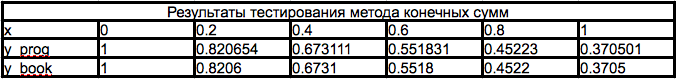
\includegraphics{Log.png} 
\textit{Рис. 1. Таблица сравнения расчетов производимых в программе и в книге.}

Следовательно метод реализован правильно и может быть в дальнейшем использован  для моделирования процессов восстановления. Под конец стоит привести скриншот программы.

На графике в зеленом спектре нарисованы смоделированные процессы восстановления для нормального распределения с заданными параметрами(в данном случае $m = 2 \sigma = 0.25$). Красным нарисовано решения интегрального уравнения.
\includegraphics*{SampleProgramm.png} 

\textit{Рис. 2. Программа после вычислений.}

\chapter*{РЕЗУЛЬТАТЫ}
\addcontentsline{toc}{chapter}{РЕЗУЛЬТАТЫ}

Далее будут приведены результаты расчетов для 1-ой и 2-ой частей, то есть для моделирования графики $H(t)$ для простых восстановлений без задержек, и графики $K_x(t)$ для альтернирующих процессов восстановлений.

\begin{center}
\item\subsection{Результаты вычислений $H(t)$ для простых процессов восстановлений}
\end{center}

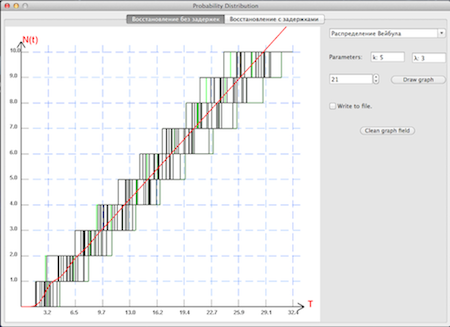
\includegraphics{3-1.png} 
\textit{Рис. 3-1. Распределение Вейбула с параметрами $k = 5$, $\lambda = 3$.}

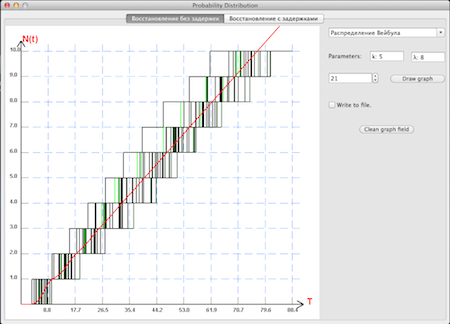
\includegraphics{3-2.png} 
\textit{Рис. 3-2. Распределение Вейбула с параметрами $k = 5$, $\lambda = 8$.}

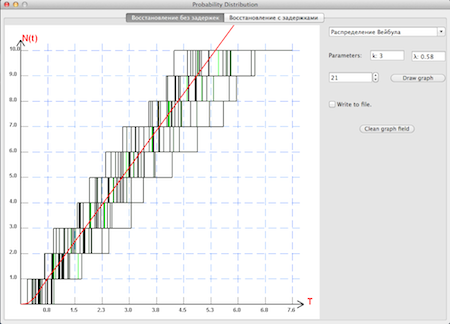
\includegraphics{3-3.png} 
\textit{Рис. 3-3. Распределение Вейбула с параметрами $k = 3$, $\lambda = 0.58$.}

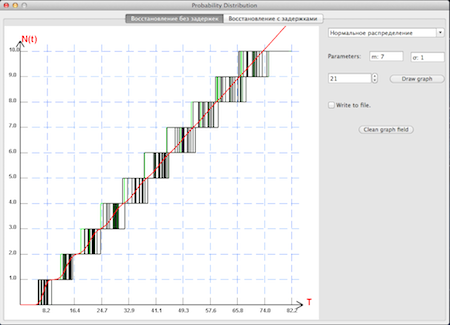
\includegraphics{3-4.png} 
\textit{Рис. 3-4. Нормальное распределение с параметрами $m = 7$, $\sigma = 1$.}

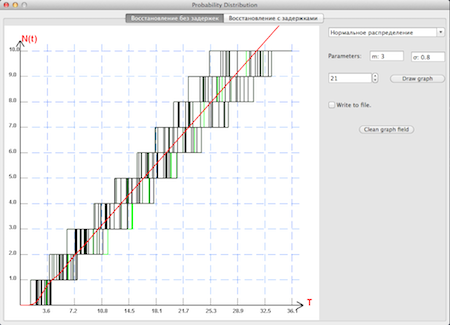
\includegraphics{3-5.png} 
\textit{Рис. 3-5. Нормальное распределение с параметрами $m = 3$, $\sigma= 0.8$.}

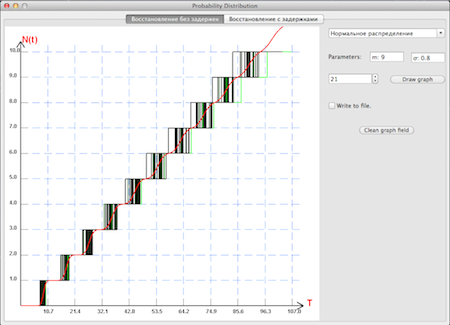
\includegraphics{3-6.png} 
\textit{Рис. 3-6. Нормальное распределение с параметрами $m = 9$, $\sigma = 0.8$.}

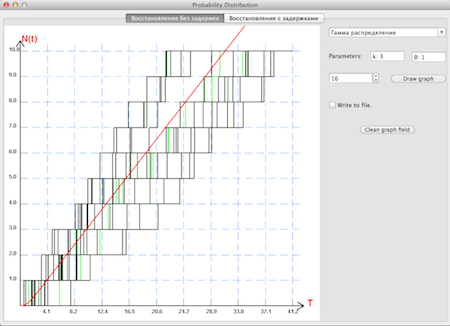
\includegraphics{3-7.png} 
\textit{Рис. 3-7. Гамма распределение с параметрами $k = 3$, $\theta = 1$.}

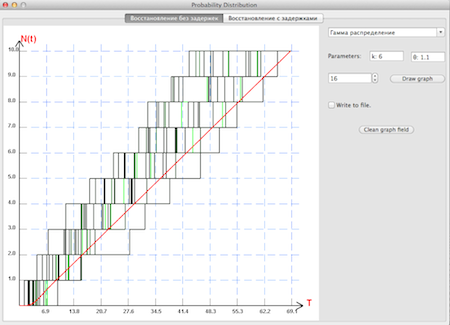
\includegraphics{3-8.png} 
\textit{Рис. 3-8. Гамма распределение с параметрами $k = 6$, $\theta = 1.1$.}

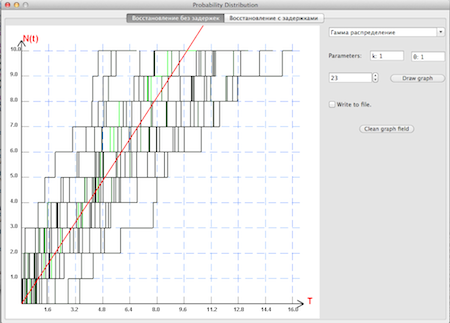
\includegraphics{3-9.png} 
\textit{Рис. 3-9. Гамма распределение с параметрами $k = 1$, $\theta = 1$.}

\begin{center}
\item\subsection{Результаты вычислений $K_x(t)$ для альтернирующих процессов восстановлений}
\end{center}

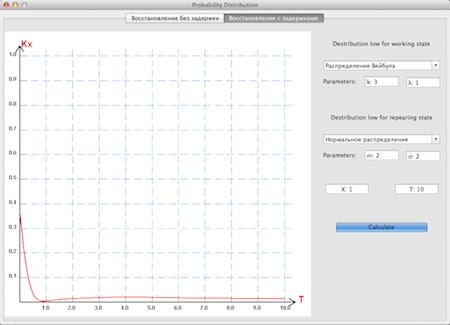
\includegraphics{4-1.png} 
\textit{Рис. 4-1. $F:$ Распределение Вейбула (3,1), $G:$ Нормальное распределение (2,2) при х = 1}

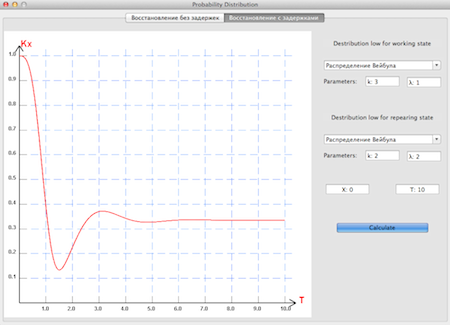
\includegraphics{4-2.png} 
\textit{Рис. 4-2. $F:$ Распределение Вейбула (3,1), $G:$ Распределение Вейбула (2,2). при х  = 0}

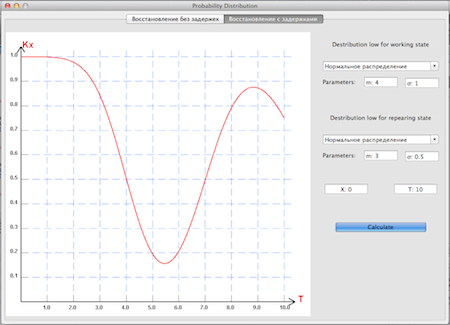
\includegraphics{4-3.png} 
\textit{Рис. 4-3. $F$:  Нормальное распределение (4,1), $G$:  Нормальное распределение (3,0.5). при х  = 0}

\chapter*{ВЫВОД}
\addcontentsline{toc}{chapter}{ВЫВОД}
В ходе двусеместрового изучения теории  восстановления были изучены основы теории восстановления и основы альтернирующих процессов восстановления. Так же было выполнено практическое задания для моделирования данных  процессов, т.е. было создано два блока программы для каждого отдельного задания на семестр.

Первый блок осуществлял расчет процесса восстановления для трех, приведенных в постановке задач, распределений. То есть он моделировал процесс восстановления и выводил его в сравнении с численным решением уравнения восстановления. Для численного решения данного интегрального уравнения использовался метод конечных сумм. В данном отчете приведен один из результатов такого вычисления, как видно из графика, уравнение восстановления достаточно точно апроксимирует полученный набор процессов восстановления. Так же для данного блока были проведены отдельные расчеты для метода конечных сумм, что помогло выявить некоторые ошибки в реализации алгоритма и впоследствии их исправить.

Для второго блока был произведен анализ новой теории, и выведена формула для 1-восстановлений $H_1(t)$. Далее был разработан второй блок программы в котором считались коэффициенты перечисленные в постановки задачи.

В итоге получилась программа реализующая два блока поставленных задач на каждый семестр. Первый блок был так же немного переделан для адаптации со вторым, но основной функционал был оставлен. Так же была изучена теория необходимая для реализации данной программы.

\chapter*{ЛИТЕРАТУРА}
\addcontentsline{toc}{chapter}{ЛИТЕРАТУРА}
\begin{enumerate}
\item  Ф. Байхельт, П. Франкен Надежность и техническое обслуживание. Математический подход: пер с нем. М.: "Радио и радиосвязь", 1988
\item Н. В. Копченова, И. А. Марон Вычислительная математика в примерах и задачах: учебное пособие. Издание второе, стереотипное. М.: "Лань", 2008
\item Д. Р. Кокс, В. Л. Смит Теория восстановления. М.: "Советское радио", 1967
\item В. И. Вайнштейн, Представление N - кратных сверток функций распределения в виде рядов и нахождение функции восстановления для некоторых
моделей процессов восстановления, М.: электронный журнал "Исследовано в России", 2005
\end{enumerate}